\chapter{TM Variants, the Church-Turing Thesis}

\begin{note}
    What kind of models are suitable for general purpose computation?
\end{note}

\section{Variants of the Turing Machine Model}

Turing machine is picked as for the general purpose computation, but choice doesn't matter, all reasonable models are equivalent in power.

\subsection{Multi-tape TMs}

Simple Turing machine has one tape, but we can also have multiple tapes.

One tape is for input, other tapes are work tapes, initially blank. All tapes can be read and write.

\begin{theorem}
    \(A\) is T-recognizable iff some multi-tape TM recognizes A.
\end{theorem}
\begin{proof}
    \begin{lemma}
        \(A\) is T-recognizable then some multi-tape TM recognizes \(A\).  
    \end{lemma}
    \begin{proof}
        This is trivial. Just use one tape.
    \end{proof}

    \begin{lemma}
        Multi-tape TM recognized \(A\) is also single tape recognizable.
    \end{lemma}
    \begin{proof}
        We can simulate multi-tape TM in single-tape Turing Machine:

        \begin{figure}[H]
            \centering
            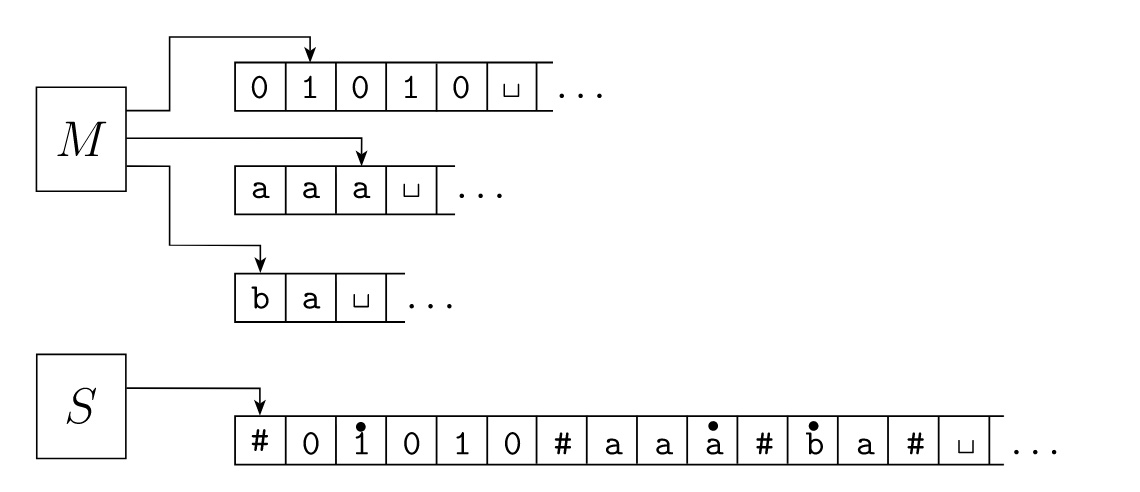
\includegraphics[width=0.8\textwidth]{f3.14.jpg}
            \caption{S simulates M}
        \end{figure}


        \(S\) simulates \(M\) by storing the contents of multiple tapes on a single tape in "block".

        Record head positions with dotted symbols, something like: \(b \rightarrow \dot{b}\) 

        If \(M\) writes to originally blank space, \(S\) has to shift room as needed. 
    \end{proof}
\end{proof}


\subsection{Nondeterministic TMs}

A \(Nondeterministic TM\)(NTM) is similar to a Deterministic TM except for its transition function \(\delta: Q \times \Gamma \rightarrow \P(Q \times \Gamma \{ L, R \} )\).

\begin{theorem}
    \(A\) is T-recognizable iff some NTM recognizes \(A\).  
\end{theorem}
\begin{proof}
    (omit the trivial direction)
    \begin{lemma}
        convert NTM to deterministic TM.
    \end{lemma}
    The lecture and the textbook use 2 different ways to simulate, I write down the proof of the lecture as it is easier to understand.

    \begin{proof}[Lecture Proof]
        The lecture simulates this using a single tape, just like the proof:

        \begin{figure}[H]
            \centering
            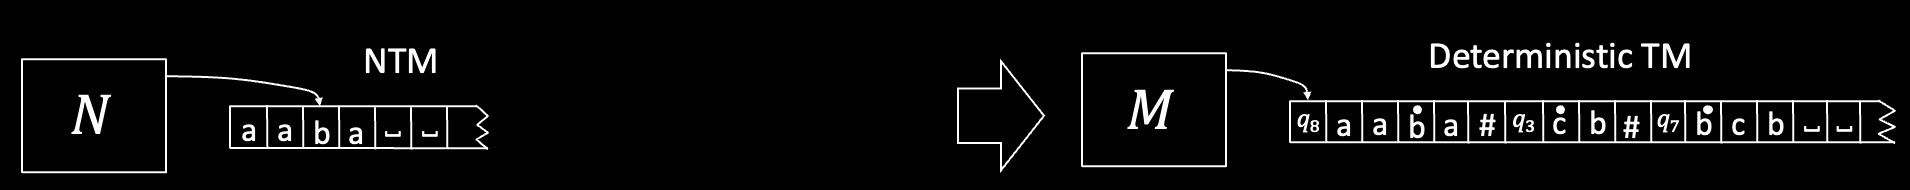
\includegraphics[width=\textwidth]{l6.1.jpg}
            \caption{M simulates N}
        \end{figure}

        \begin{itemize}
            \item \(M\) simulates \(N\) by storing each thread in separate "block"
            \item Also need to store the head location
            \item Need to store status of each thread
            \item If a thread forks, then \(M\) copies the block
            \item If a thread accepts then \(M\) accepts.    
        \end{itemize}
    \end{proof}
\end{proof}

\subsection{Enumerators}

\begin{definition}[informal]
    A \underline{Turing Enumerator} is a deterministic TM with a printer. The Turing machine can use that printer as an output device to print strings. Every time the Turing machine wants to add a string to the list, it sends the string to the printer.
\end{definition}

\begin{figure}[H]
    \centering
    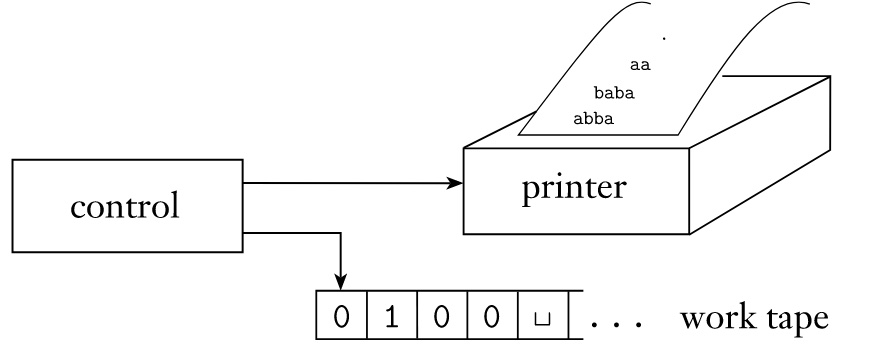
\includegraphics[width=0.8\textwidth]{f3.20.jpg}
    \caption{Schematic of an enumerator}
\end{figure}

The enumerator \(E\) starts with a blank input on its work tape. The language enumerated by \(E\) is the collection of all the strings that it eventually prints out.  

\begin{theorem}
    \(A\) is T-recognizable iff \(A = L(E)\) for some T-enumerator E. 
\end{theorem}
\begin{proof}
    \begin{lemma}
        Convert \(E\) to equivalent TM \(M\): If we have an enumerator \(E\) that enumerates a language \(A\), a TM \(M\) recognizes \(A\).     
    \end{lemma}
    \begin{proof}
       The TM \(M\) works in the following way:
         
       \(M = \)" On input \(w\):
       \begin{enumerate}
        \item Run \(E\). Every time that \(E\) outputs a string, compare it with \(w\).
        \item If \(w\) ever appears in the output of \(E\), \(accept\)."    
       \end{enumerate}

       Clearly, \(M\) accepts those strings that appear on \(E\)'s list.  
    \end{proof}

    \begin{lemma}
        If TM \(M\) recognizes a language \(A\), we can construct the following enumerator \(E\) for \(A\).    
    \end{lemma}
    \begin{proof}
        Say that \(s_1, s_2, s_3, \cdots\) is a list of all possible strings in \(\Sigma^*\). 

        \(E = \) "Ignore the input.
        \begin{enumerate}
            \item Repeat the following for \(i = 1, 2, 3, \cdots\) 
            \item Run \(M\) for \(i\) steps on each input, \(s_1, s_2, \cdots, s_i\)
            \item If any computations accept, print out the corresponding \(s_j\)" 
        \end{enumerate} 

        \begin{intuition}
            This is basically the E uses the TM it attaches to recognize the language, and print if the attached TM recognizes it.

            It can be an infinite loop because all possible strings in \(\Sigma^*\) is infinite if it does not only contain \(\epsilon\).  

            But when really run the TM, we have to run in parallel, as the TM might be looping.
        \end{intuition}
    \end{proof}
\end{proof}

The essential feature of TM is \textit{unrestricted access to unlimited memory}, it distinguishes TMs from other weak models. Some other models also have the same power as TMs, and they also share the same feature.

\section{Church-Turing Thesis}

\begin{remark}
    \textit{Intuitive notion of algorithms}    
    \quad 
    equals 
    \quad 
    \textit{Turing machine algorithms}
\end{remark}

Church used a notational system called the \(\lambda-\)calculus to define algorithms. Turing did it with his "machines". The two definitions where shown to be equivalent. The connection between the informal notion of algorithm and the precise definition has come to be called \textit{\textbf{Church-Turing thesis}}.

It has been used by Yuri Matijasevi to solve Hilbert's 10th problem:

\begin{quotation}
    to provide a general algorithm that, for any given Diophantine equation (a polynomial equation with integer coefficients and a finite number of unknowns), can decide whether the equation has a solution with all unknowns taking integer values.(\href{https://en.wikipedia.org/wiki/Hilbert%27s_tenth_problem}{Wikipeadia: Hilbert's tenth problem}) 
\end{quotation}

\begin{note}
    The idea is to prove the language of Diophantine equations is TM recognizable but not decidable.
\end{note}

\section{Notation for encodings and TMs}

We're going to accept more types (even automaton) as input to Turing machine. But TM only accepts strings, so we need to encode objects into strings.

- If \(O\) is some object, we write \(\langle O \rangle\) to be an encoding of that object into a string.  

- If \(O_1, O_2, \cdots, O_k\) is a list of objects then we write \(\langle O_1, O_2, \cdots, O_k \rangle\)  to be an encoding of them together into a single string. 

